\documentclass[10pt,letterpaper]{article}

\usepackage{cogsci}
\usepackage{pslatex}
\usepackage{apacite}
\usepackage{graphicx}
\usepackage{caption}
\usepackage{subfigure}
%\usepackage{subcaption}
\usepackage{subfigure}
\graphicspath{{figures/}}
  
\usepackage{color}

\definecolor{Red}{RGB}{255,0,0}
\newcommand{\red}[1]{\textcolor{Red}{#1}}  
  
\usepackage{listings}
%\usepackage{inconsolata}
\usepackage{xcolor} %to use colored text

\lstset{
language=Scheme,
basicstyle=\footnotesize\ttfamily,
mathescape=true,
frame=single
}

\begin{document}

\title{Some arguments are probably valid: Reason and language in syllogisms}
 
\author{{\large \bf M. H. Tessler, Noah D. Goodman } \\
	\{mhtessler, ngoodman\}@stanford.edu \\
  Department of Psychology, Stanford University}

\maketitle


\begin{abstract}
We develop a computational-level theory of syllogistic reasoning which places reasoning at the intersection of communication and logic. We compare our model predictions with behavioral data from a recent meta-analysis. We show the flexibility of the model to account for reasoning behavior in a study of so-called ``statistical syllogisms" which use the generalized quantifiers \emph{most} and \emph{few}. We relate our model to three extant theories of syllogistic reasoning -- Mental Models, Mental Logics and Probability Heuristics. We conclude by discussing further predictions of the model and future directions.  
\\
\textbf{Keywords:} 
Reasoning, language understanding, probabilistic model
\end{abstract}


Consider for a moment that your friend tells you:
``Everyone in my office has the flu and, you know, some people with the flu are out for weeks.''
Do you respond with
``Everyone in your office has the flu.''
Do you respond with
``Pardon me, there is no inference I can draw from what you just said."
Or do you respond
 ``I hope your officemates are not out for weeks and I hope you don't get sick either."
 The first response is true, but does not go beyond the premises; the second response attempts to go beyond the premises by strict classical logic, but fails; the final response goes beyond the premises, to offer a conclusion which is probably useful and probably true.
% 
This cartoon illustrates two dimensions along which cognitive theories of reasoning differ: whether the core and ideal of reasoning is deductive validity or probabilistic support, and, the natural language principles---pragmatics and semantics---for understanding reasoning. In this paper we explore a theory of syllogistic reasoning inspired by recent advances in probabilistic semantics and pragmatics.

The form of the argument above resembles a syllogism: an argument with two quantifier expressions (premises) used to relate two properties (or terms) via a middle term. Fit into a formal syllogistic form, this argument would read:
\begin{quote}
All officemates are out with the flu\\
Some people out with the flu are out for weeks\\
\end{quote}
The full space of syllogistic arguments is derived by shuffling the term-ordering (``All A are B'' vs. ``All B are A'') and changing the quantifier (\emph{all, some, none, not all}). Most syllogisms have no valid conclusion, i.e. there is no deductive relation between A \& C determined by the premises. This is the case with the argument above. A recent meta-analysis of syllogistic reasoning tasks showed that over the population, accuracy on producing valid conclusions ranges from 90 \% to 1\% and ability to produce appropriate \emph{no valid conclusion} responses ranges from 76\% to 12\% \cite{khemlaniJL2012}: people are not good at drawing deductively valid conclusions.
%
Perhaps because of this d\'ecolage between human behavior and deductive logic, syllogistic reasoning has been a topic of considerable interest in cognitive psychology for over one hundred years \cite{storring1908}, and before that in philosophy, dating back to Aristotle. In cognitive psychology we are interested in how people reason, and syllogisms lie at the intriguing intersection of natural and formal reasoning, of  language and logic. They are undoubtedly logical; indeed, they are regarded as the first formal system of logic. At the same time, they use natural language quantifiers and invite natural language conclusions; precisely pinning down the meaning and use of quantifiers has been an ongoing area of inquiry since Aristotle \cite<e.g.>{negationHorn}.


Many theories of syllogistic reasoning take deduction as a given and try to explain errors as a matter of errors in the system. These error may arise from improper use of deductive rules, or biased construction of logical models. In either case, logic makes the connection to natural language semantics natural (though not central).
On the other hand, many other kinds of reasoning have been explained via probabilistic reasoning under uncertainty. Probability provides a natural description of a world in which you don't know how many people are in the hallway outside your door or whether or not the lion is going to start charging.
We will suggest that combining probabilistic reasoning with formal semantics and pragmatics of natural language leads to a useful combination of these approaches, in which our knowledge describes distributions on possible situations and sentences naturally update these distributions with new information.
In this formalism, deduction emerges as those arguments which are always true and syllogistic reasoning becomes a process of determining what is most probable, relevant, and informative.


%
%Theories of syllogistic reasoning have been  One possibility is {\emph{logical deduction}. When a theory takes deduction to be fundamental, the explanatory power of the theory derives from explaining errors in deductive inference. That is to say, these theories treat the variety of performance errors as the first-class explanandum.
%
%We take a different path. We propose, as has been proposed before, that people are reasoning according to their {\emph everyday} mode of reasoning. {\emph Everyday} reasoning is understood as the type of reasoning that is refined for dealing with a world of uncertainty, a world in which you don't know how many people are in the hallway outside your door or whether or not the lion is going to start charging. This type of reasoning is most succinctly described in the language of probability theory. 

\section{The Conditional Semantics model}

The motivation for our model stems from the intuitions that people reason by constructing situations consistent with their probabilistic prior knowledge, and they interpret premises and choosing conclusions as 


: (1) people are using \emph{everyday} reasoning in syllogistic reasoning tasks and (2) they do this by constructing situations and reasoning about these situations. For syllogistic reasoning, it is natural to think of situations as composed of objects with properties\footnote{These situations are not entirely different from Johnson-Laird's notion of a {\emph mental model}, which we discuss later. We prefer the term situation so as to not confound the word model, which we take to refer to a computational model.}. In a probabilistic model, situations arise from a sampling procedure.

Situations are composed of $n$ number of objects, each with 1, 2 or 3 properties corresponding to the three terms of a syllogism. Situations are sampled from a naive prior. In this setting, it is reasonable to assume that the prior probability, $P(situation)$, is a binomial distribution (i.e. the probability of a coin of a given weight coming up Heads $n$ times in a row, where $n$ is the number of objects). We assume properties are relatively rare of objects; this means the base rate (br) of properties is less than 0.50.  This principle of rarity comes from the intuition that properties are relative rare \footnote{This article is an article and it's about reasoning, but it's not a cat, and it's not a car, nor an elephant nor the color red. In fact, there's a very large number of things which this article is not.}, and this has been used in probabilistic models previously. 

\begin{lstlisting}
(define A (mem (lambda (x) (flip br))))
(define B (mem (lambda (x) (flip br))))
(define C (mem (lambda (x) (flip br))))
\end{lstlisting}


To reason over situations, we draw on ideas in formal semantics by assuming that propositions are truth-functional operators. A given proposition (e.g. {\emph All As are Bs} is a function which takes in a situation and returns a truth value. From this we get a prior distribution over propositions. By sampling over many situations, we construct a distribution over propositions, shown in Figure 1, first column.

\begin{lstlisting}
(define all (lambda (x) (eval-all x)))
(define some (lambda (x) (eval-some x)))
...
\end{lstlisting}

The Conditional Semantics model treats the premises of a syllogism as evidence by which to update its belief prior over propositions (which are now potential conclusions). This update rule we take to be probabilistic conditioning. Thus, we get a posterior distribution of propositions, conditioned on premises being true. This has the nice feature of returning a degree of belief in each of the possible conclusions for every syllogism. Using this, we can test the hypothesis that reasoners in syllogistic reasoning tasks are essentially drawing samples from the posterior distribution of the conclusion conditioned on the premises (so-called ``posterior matching")\cite{Griffiths2006}.

\begin{lstlisting}
(query
  ...define A,B,C...
  (define conclusion (conclusion-prior))
  
  conclusion
  
  (and (conclusion A C)
  	 (premise-one A B)
     (premise-two B C))
\end{lstlisting}


\subsection{Conditional Pragmatics}
One reason to be skeptical of mere \emph{posterior matching} in syllogistic reasoning is that language understanding and language production are central to the syllogistic task, and truth-functional semantics can only go so far. It is natural to think of natural language pragmatics as entering in two places in the model: premise interpretation and conclusion production. We address only production in the current model \footnote{Preliminary analyses suggest standard Gricean implicatures are not all that's at play during premise comprehension. This is consistent with other empirical findings which set out to test this. We address this matter in more detail later.}. To illustrate pragmatic production, we offer as an example the canonical ``All/all" syllogism:

\begin{quotation}
All As are Bs \\
All Bs are Cs \\
\end{quotation}

This is in fact one of the easiest syllogisms to which 81\% of participants produce the valid{\emph All As are Cs} conclusion. The other valid conclusions -- \emph{Some As are Cs} and \emph{Some Cs are As} receive only 7\% of the endorsements. However, in every possible situation in which {\emph All As are Cs} is true, \emph{Some As are Cs} and \emph{Some Cs are As} are also true. That is, they are equally probable given the posterior. 

This illustrates one of the issues with the conditional semantics model: it is too literal. The model computes the probability of the conclusion conditioned on the premises being true. For logically valid syllogistic conclusion, this probability is equal to 1. In particular, for any syllogism for which one of the universal quantifiers is valid (i.e. {\emph all} and {\emph none}), the particular quantifier (i.e.{\emph some} and {\emph not all}, respectively) will also be valid. Human reasoners show a clear preference for conclusions using universal quantifiers (all and none) in these cases. 

To address this we draw on recent advances in probabilistic models of pragmatic reasoning. The \emph{rational speech-act theory} addresses the problem of language understanding as that of a speaker trying to convey information about a world or situation that the speaker has observed \cite{Frank2012a}. The speaker draws on common-ground of communicative goals to maximize information content of a given utterance. In particular, choosing an utterance in proportion to the likelihood of a listener inferring the situations about which the speaker wishes to convey information. In turn, a listener considers situations in which the given utterance heard is not only true but would be chosen to disambiguate amongst multiple consistent situations by an informatve speaker. This results in the canonical ``scalar implicature" wherein the literal meaning of ``{\em some} of the apples are red" is enriched to communicate ``some {\em but not all} of the apples are red".

We use a variant of the nested-conditioning model of scalar implicature \cite{Goodman2013} to break the symmetry described above. We treat the reasoner as a sort of pragmatic speaker with a hypothetical listener in the reasoner's mental representation. This listener can be thought of concretely as the person evaluating the participant's responses. In the original scalar implicature model, the listener hears an utterance and tries to reconstruct the situation observed by the speaker. In our model, the listener hears the conclusion and tries to reconstruct the premises with which the reasoner was presented. This distinction turns out to be important as the reasoner does not observe a situation directly but rather constructs situations consistent with the premises. 

\section{Results}

\subsection{Meta-analysis data}
To test our model, we used data from the meta-analysis presented with the Probability Heuristics Model\cite{Chater1999}. These data were compiled from 5 studies on syllogistic reasoning, completed from 1978-1984. The data included percentage response for conclusions of each of the 4 quantifiers as well as ``No Valid Conclusion". We consider the production of the ``No Valid Conclusion" an aspect of the algorithmic implementation and leave this for future work. The meta-analysis includes studies for which both conclusion orderings were allowed (A-C or C-A). Because of this, we allowed our model to do the same. Following the procedures of the meta-analysis, we collapsed responses across these two orderings to compare it to the data set.

\subsection{Model fit}
For each model, we report the total number of syllogisms the model's model response is the same as for the meta-analysis. This is a qualitative assessment of the fit. We compute correlations across all 256 data points (64 syllogisms x 4 conclusions) to assess the overall fit quantitatively. 

We first examined the prior to see if it alone accounted for human reasoning patterns. It did not. Since ``not all" is the most likely conclusion to be true, the prior gets only the syllogisms with a ``Not all" modal response correct. For the meta-analysis data, this amounts to 29 out of the 64 syllogisms. The overall fit is also accordingly poor (r = .36). 

When we condition on the premises being true, the model matches people's maximum judgments on 37 of the 64 syllogisms. This includes all of the syllogisms for which ``not all" is the modal response, as well as 8 syllogisms for which ``some" and ``none" are favored. The overall correlation is accordingly higher (r=0.64). However, among valid conclusions the correlation is terrible (r=0.05). This is a direct consequence of the model's literalness. Among valid conclusions to valid syllogisms, the model has no preference.

By introducing pragmatics to the model, we are able to distinguish among equally ``certain" conclusions. The model selects not only conclusions likely to be true, but conclusions which are informative to a hypothetical listener. The model now matches 44 out of 64 modal responses and has a correlation of r = 0.77. The difference is especially striking for the valid syllogisms, for which the correlation is now r = 0.85. We compared these results to those found when using a uniform prior and found the overall fit much better with the binomial, which invokes the principle of rarity. 

\begin{figure*}[t!] %[htp]
\centering
	\subfigure
		\centering
  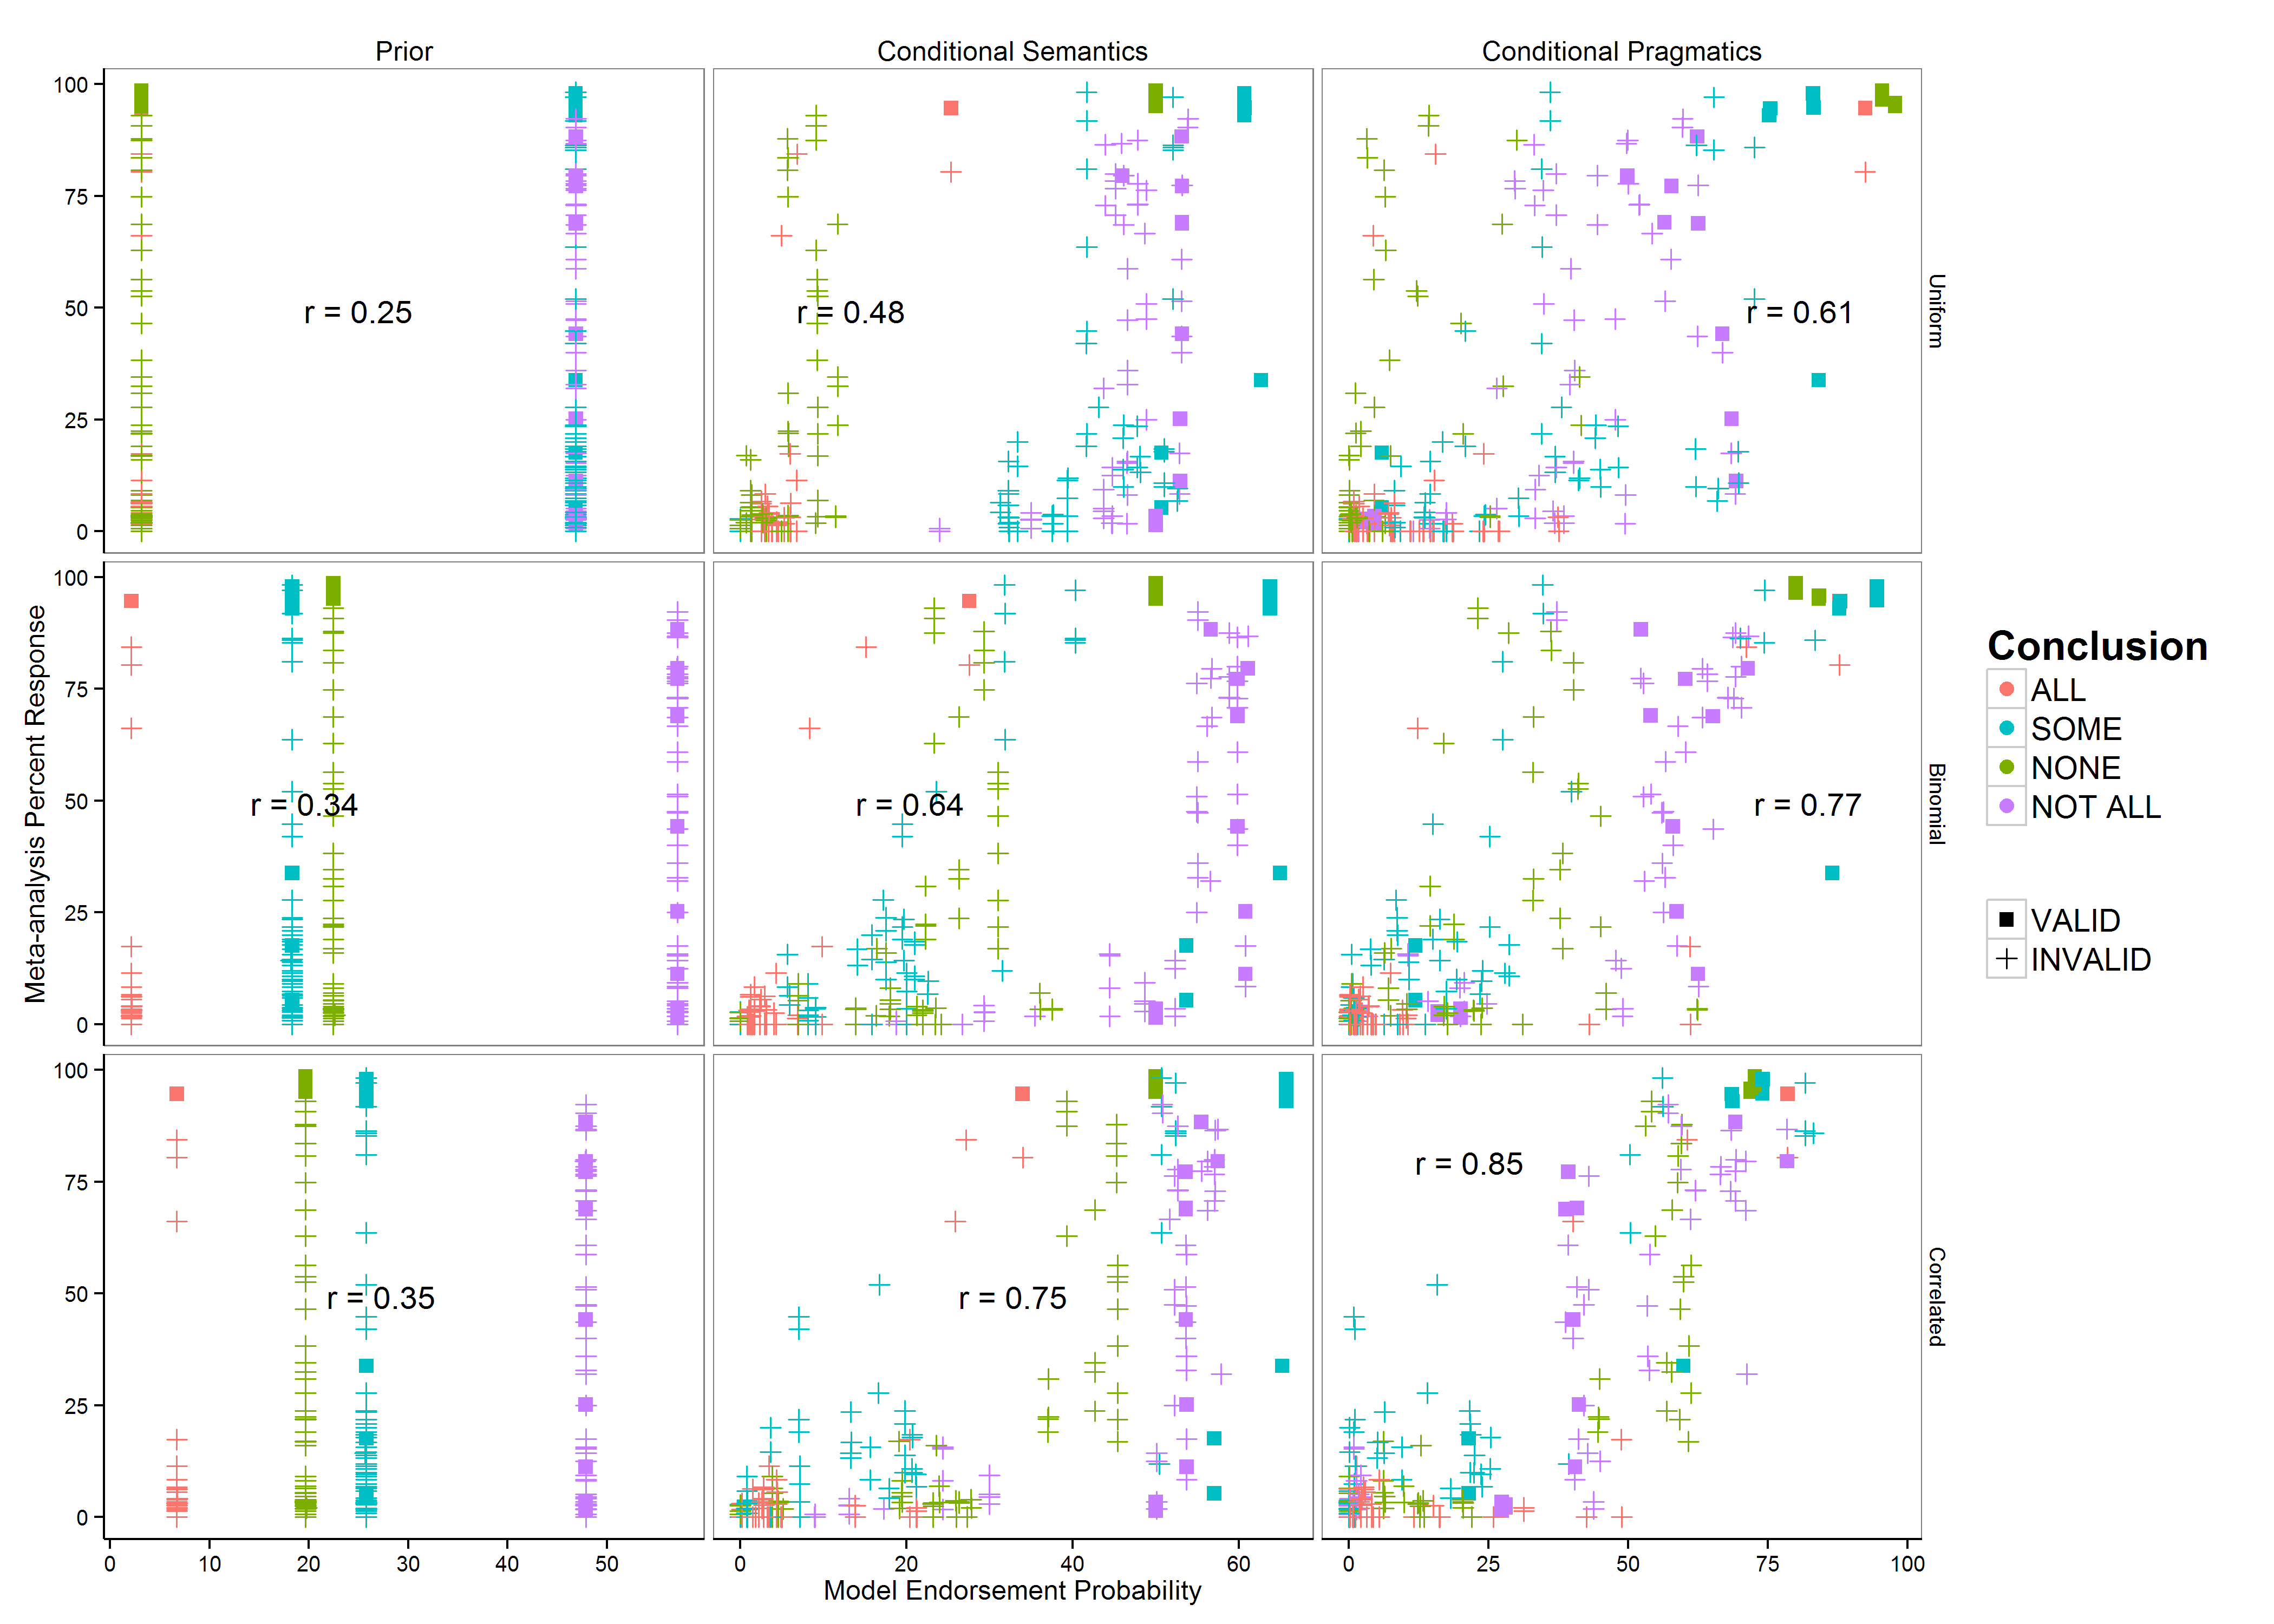
\includegraphics[width=\textwidth,height=10cm]{multiScatter_unif-bin-2m40br_n6_alphabefore2}
  \caption{Human subject percentage endorsement vs. model fits for 3 different priors. Columns, from left to right: models based only on the prior, Conditional Semantics models, and Conditional Pragmatics models. Rows from top to bottom: uniform prior, binomial prior, conditional prior (see text).}
  \label{fig:megaScatter}
\subfigure

    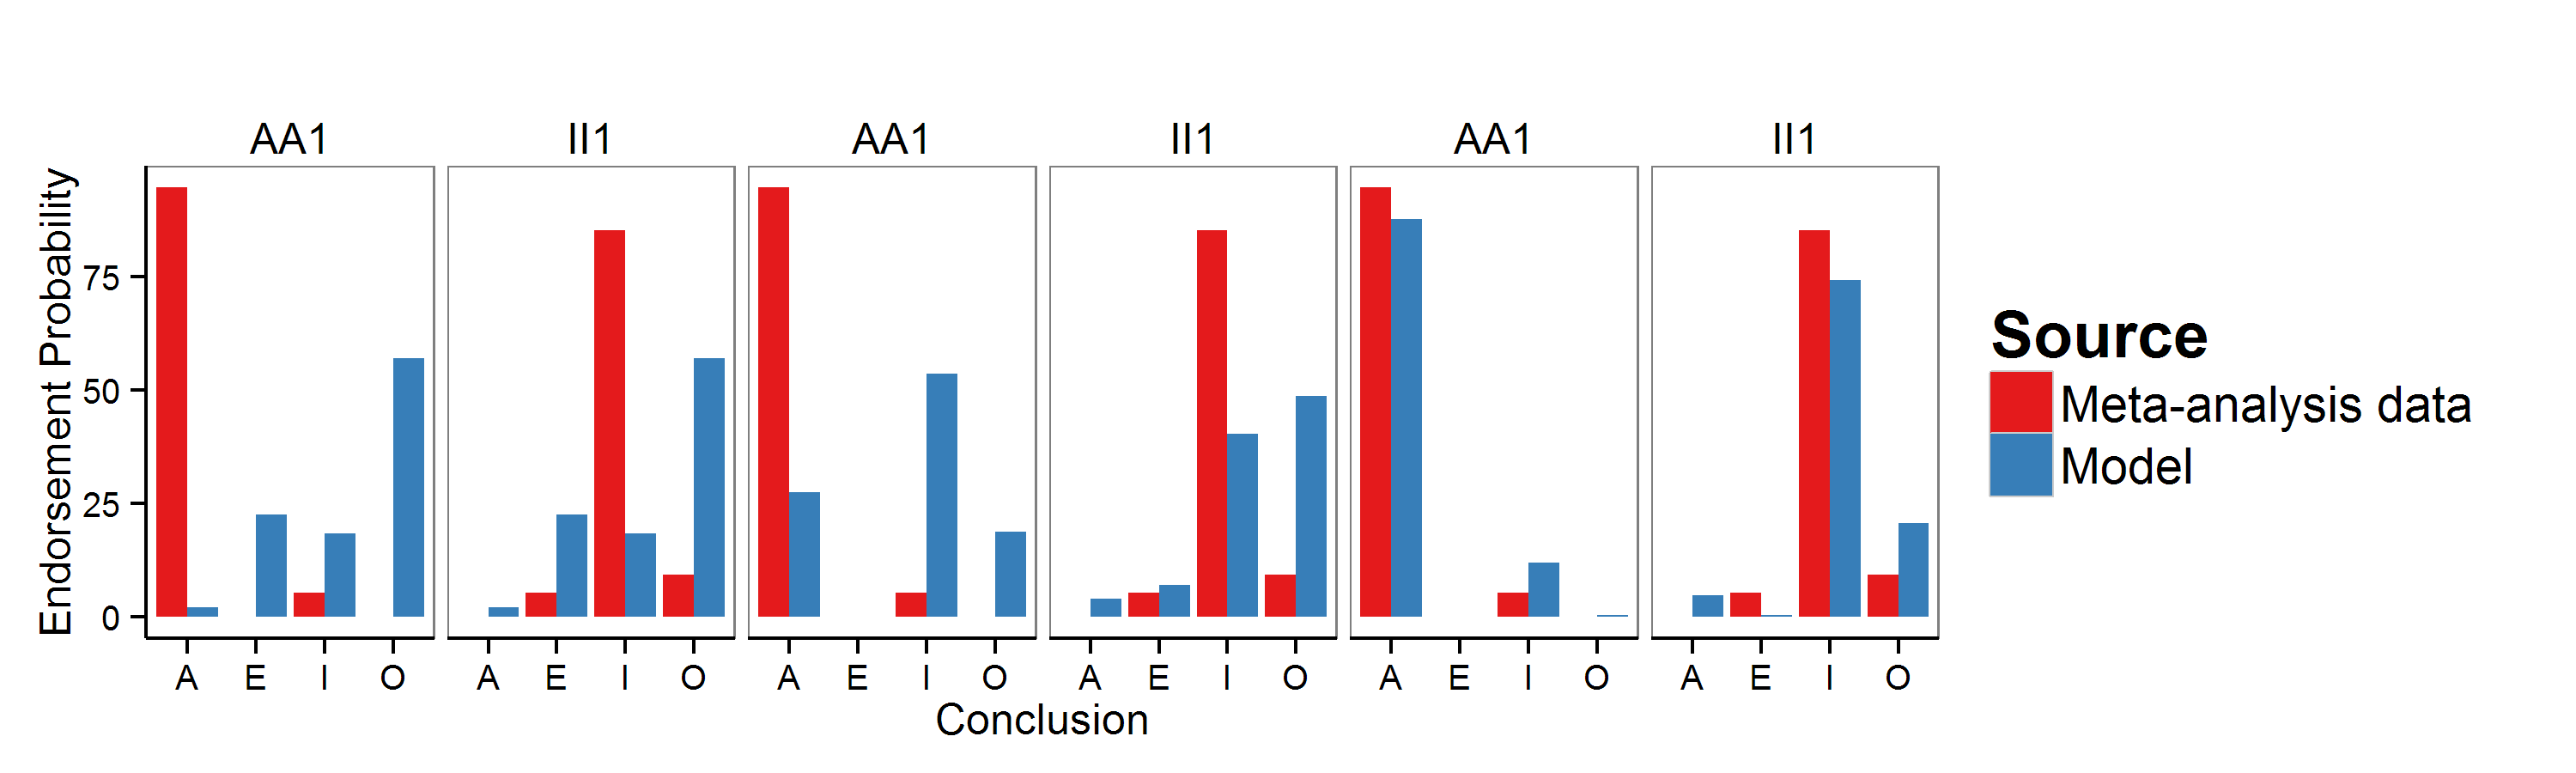
\includegraphics[width=\textwidth,height=4cm]{multibar_AA1_II1_luceSpeak2}
    \caption{Two example syllogisms. Pragmatic effects both strengthen already likely conclusions as well as relatively unlikely but informative conclusions.}
  \label{fig:barplots}

\end{figure*}

\subsection{Dependency}

The inspiration for this model comes from the idea that syllogistic reasoning can not be disentangled from language understanding. In particular, natural language semantics is insufficient to explain the variability in such a data set. We argue that understanding conversational pragmatics is necessary to understanding how people reason with syllogistic arguments. We have found that the meanings of quantifiers are important insofar as \emph{some} might imply \emph{not all} and so people prefer to conclude \emph{all} when it is warranted. 

We speculate that there is another important pragmatic effect which dominates the interpretation of the premises. In what natural setting does a person produce a syllogistic like argument? Why would anyone ever go through the hassle of uttering two sentences which do not convey the totality of what is intended to be conveyed? We suggest this is due to an asymmetry among the three relations (i.e. A-B, B-C, C-A). We posit that the A-B \& B-C relations are weighted more strongly than the A-C relationship, possibly owing to common ground of those relationships. In some way, A-C is unexpected, or somewhat unbelieveable. If it weren't, there would be no reason to work through the syllogism. The syllogism was invented as a tool of argument, to convince others. Nobody needs convincing that ``Socrates is mortal". 

Following up on this intuition, we introduced a small dependency (df) into the binomial prior such that A \& C are more likely when B is present and less likely when B is absent. In our example from the beginning, this means that some of your office mates being out of the office for weeks is less likely if they don't have the flu and more likely if they do have the flu. 


\begin{lstlisting}
(define B (mem (lambda (x) (flip base_rate))))
(define A 
  (mem (lambda (x) 
    (flip (if (B x) (+ br df) (- br df))))))
(define C 
  (mem (lambda (x) 
    (flip (if (B x) (+ br df) (- br df))))))
\end{lstlisting}

Using this conditional prior, the Conditional Semantics model gets 45 out of 64 modal responses. The overall fit is also improved, r = 0.75. The Conditional Pragmatics model does better as well, predicted the modal response for 52 syllogisms. Additionally, the quantitative fit is high (r = 0.85). Among valid syllogisms, it is correspondingly higher as well (r = 0.88). 


\section{Most and few}

Our model is based on a truth-functional semantics and as such, it is able to accommodate any quantified sentence with a truth-functional meaning. The question of the meaning of generalized quantifiers like ``most" and ``few" is a topic of great interest to the field of formal semantics. Often, ``most" and ``few" are modeled by a thresholded step function. As a first test of the generality of the model, we define most and few by a threshold of 0.5 such that ``most As are Bs" is true if more than half of the As are Bs. We realize this is a gross oversimplification of the meanings of these words. We maintain the set size parameter of 6. However, we feel the usage of the words ``most" and ``few" might bias people to represent sets of larger size.

We compare our model predictions to two studies carried out by Chater \& Oaksford on syllogisms using generalized quantifiers. In these studies, participants were given syllogisms with these generalized quantifiers e.g. {\emph Most artists are beekeepers. Few chemists are beekeepers.}. Participants were told to indicate which, if any, of the four conclusions followed from the premises and were allowed to select multiple options.

The set of all possible syllogisms with 6 quantifiers contains 144 questions.  The authors divided these into two experiments to avoid subject fatigue. Experiment One consisted of the \emph{all},\emph{not all},\emph{most}, and \emph{few} quantifiers. Experiment Two used \emph{most},\emph{few},\emph{some}, and \emph{none}. 

\begin{figure*}[ht]
	\centering
	\subfigure

  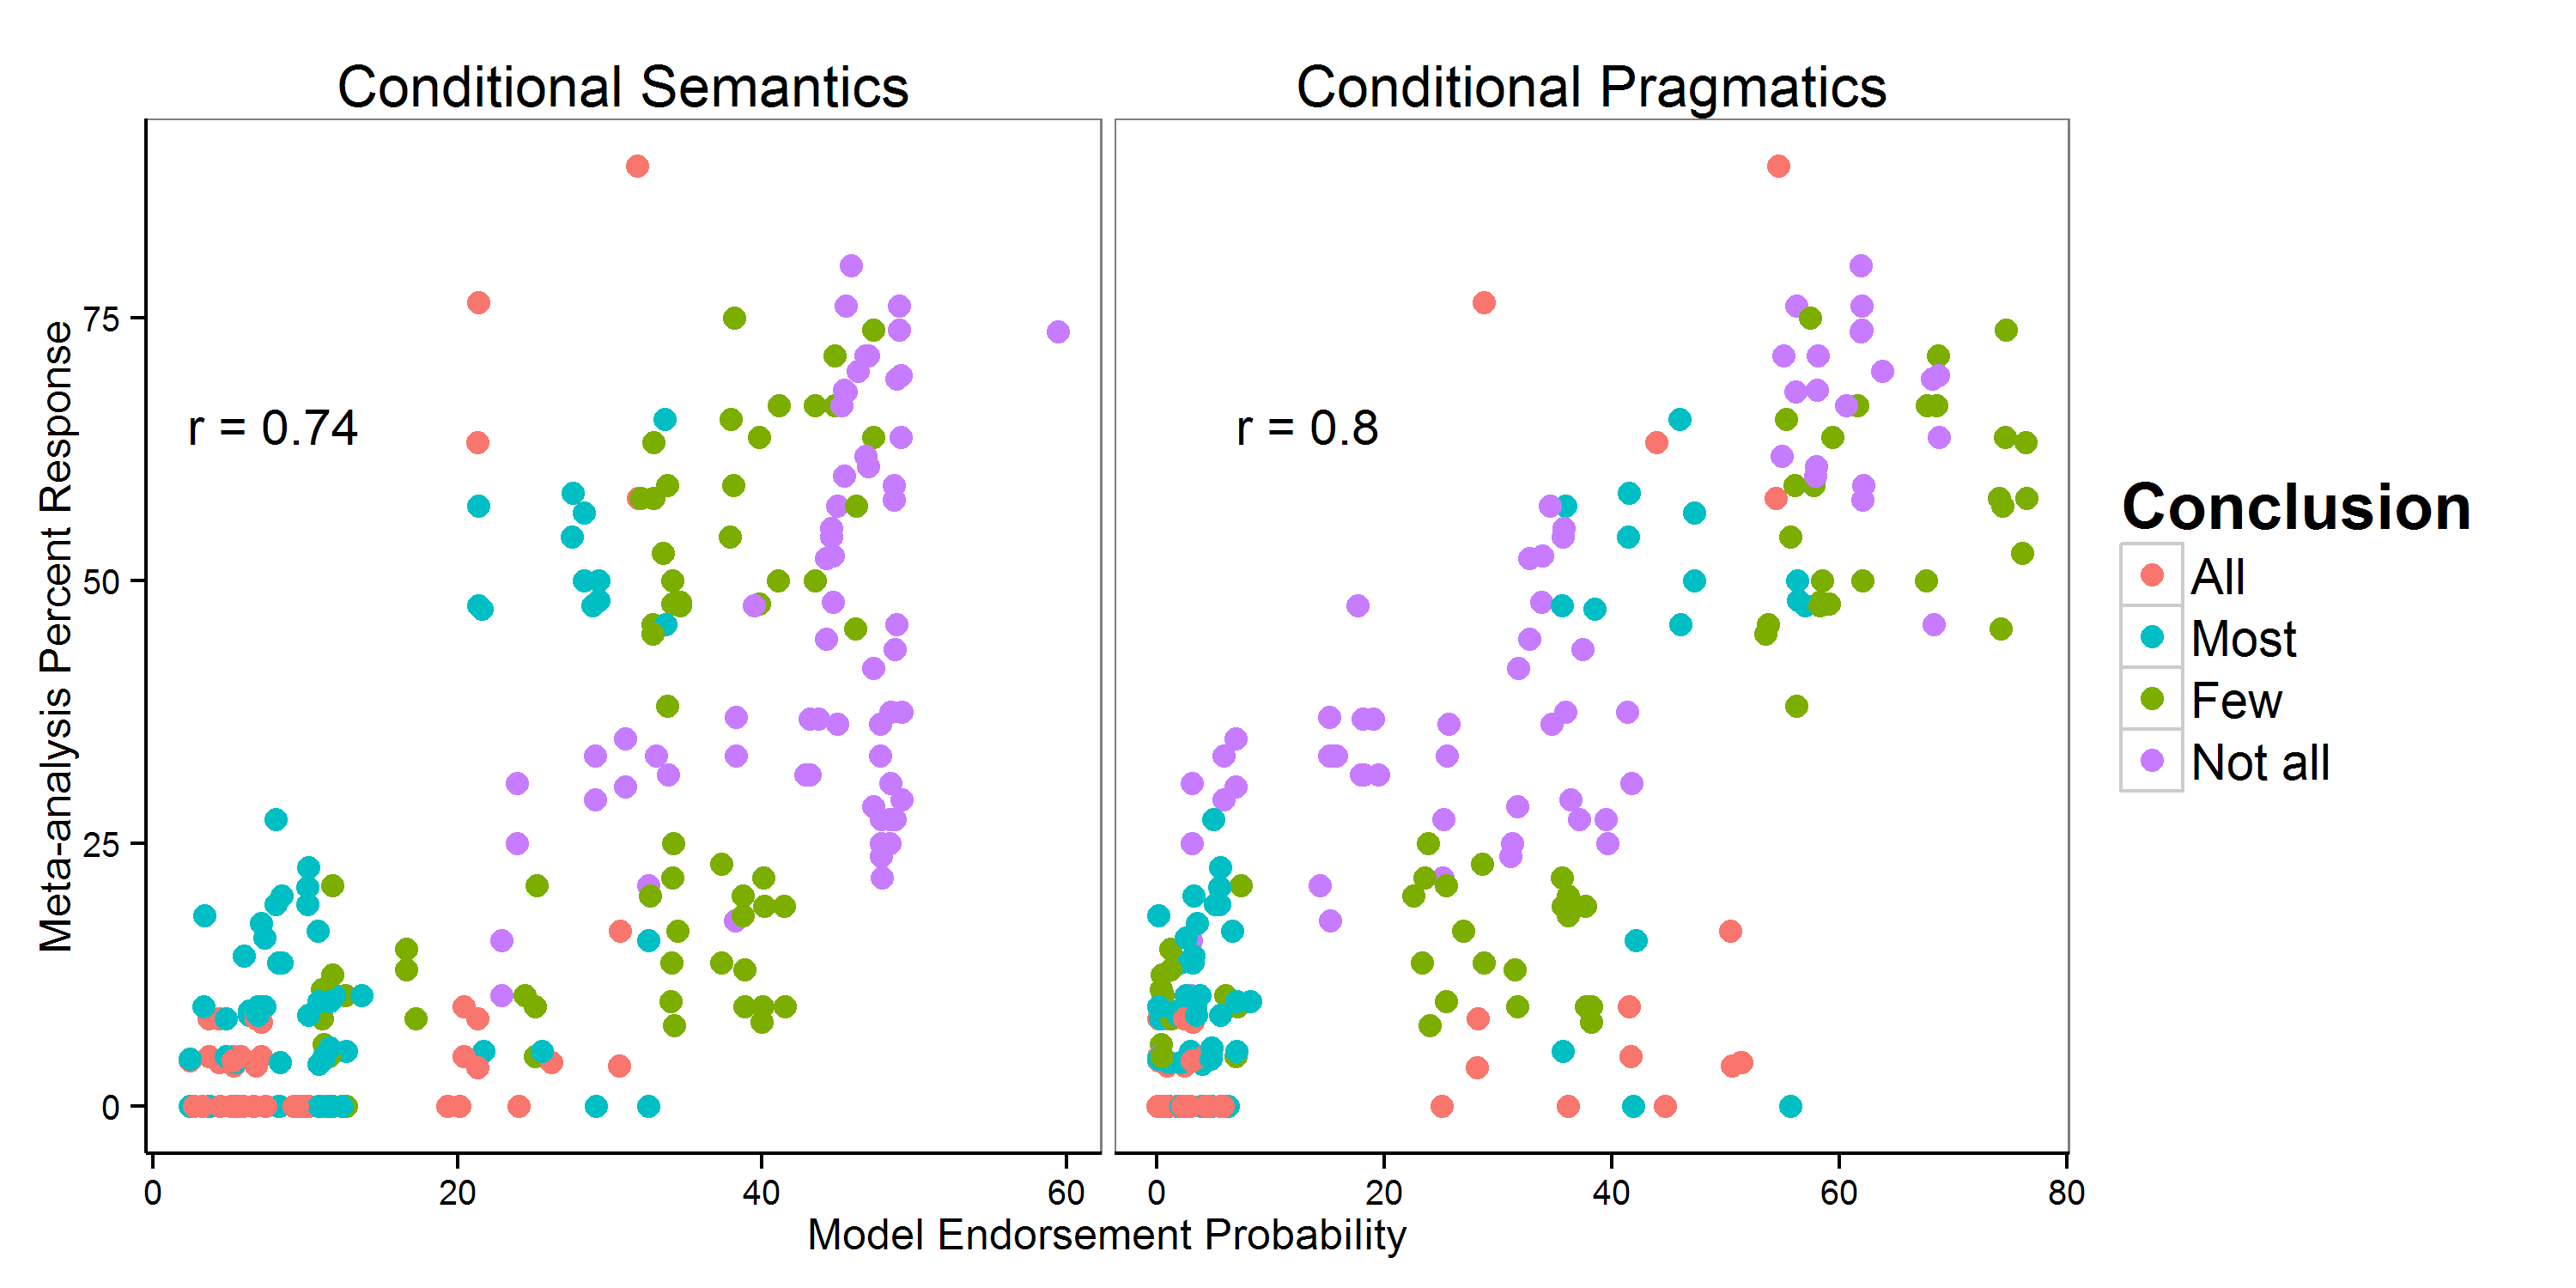
\includegraphics[width=10cm,height=4cm]{multiScatter_AMFO_n6_alphabefore1}

  \label{fig:amfoScatter}
\subfigure
	\centering
    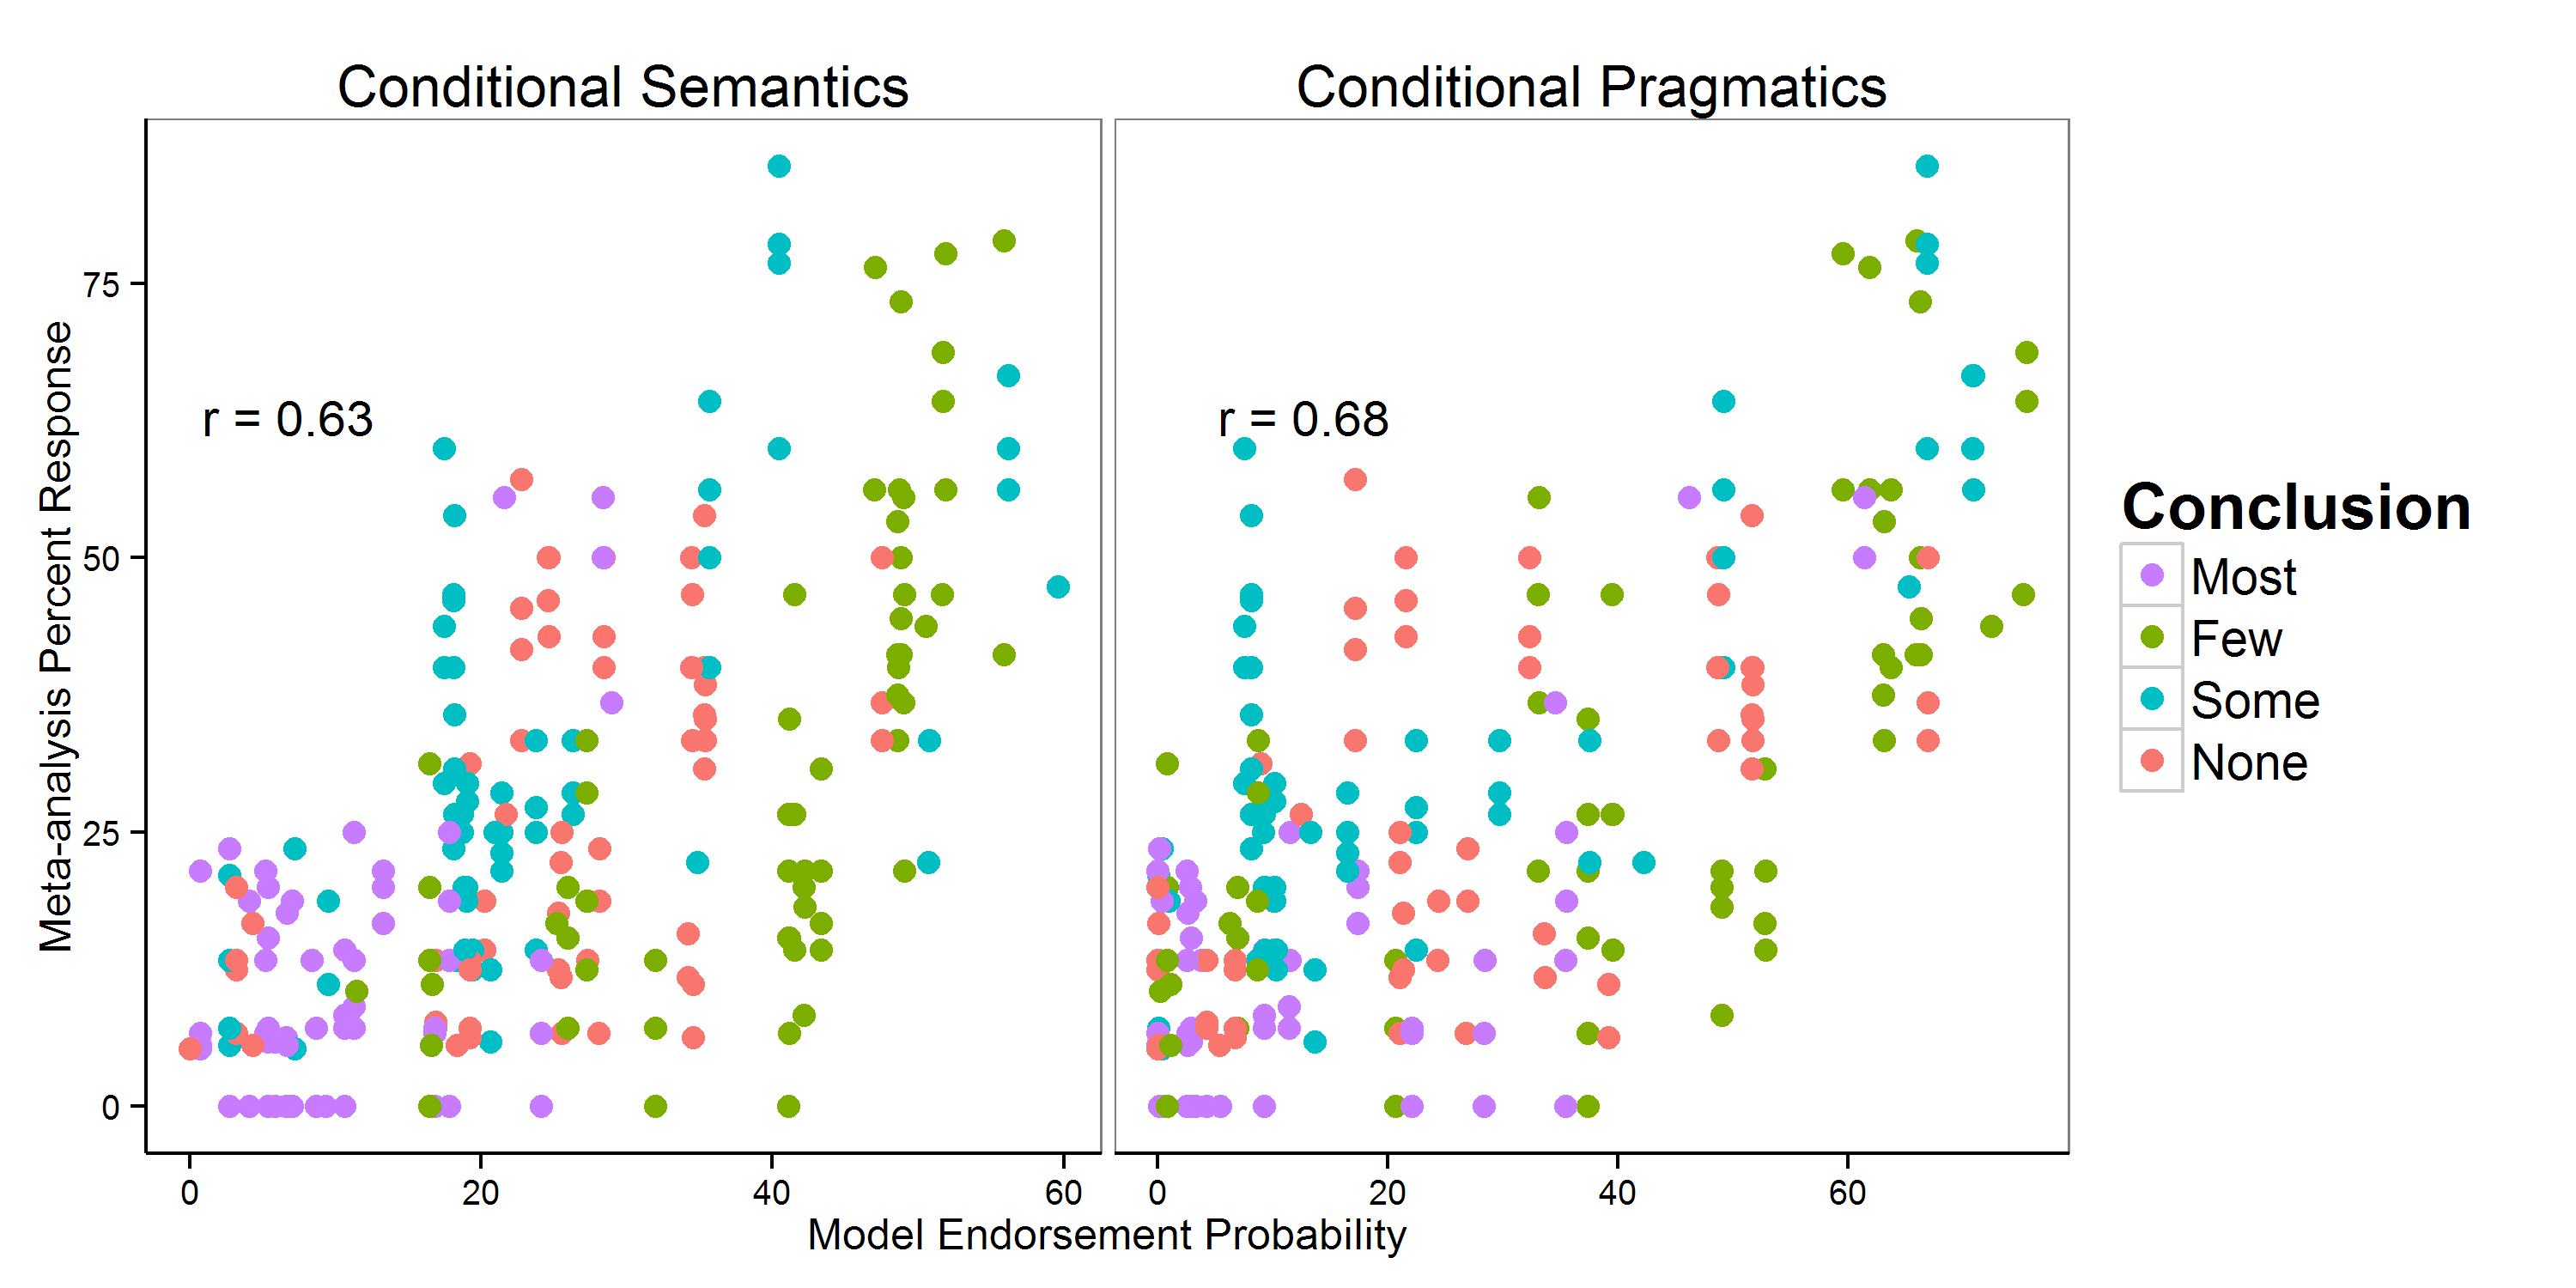
\includegraphics[width=10cm,height=4cm]{multiScatter_MFIE_n6_alphabefore1}
      \caption{Human subject percentage endorsement vs. model fits for 2 experiments using generalized quantifiers. Predictions for the Conditional Semantics model is on the left. Predictions for the conditional pragmatics model is on the right.}
  \label{fig:mfieScatter}
\end{figure*}


We find good correspondence between the experimental data and the model, even without doing any parameter fitting. The fit is better for the experiment using \emph{all},\emph{most},\emph{few}, and \emph{not all} (r = 0.80) than for the experiment using \emph{most},\emph{few},\emph{some}, and \emph{none} (r = 0.68). The same was true for the Probability Heuristics Model (r = 0.94 vs r = 0.63). Overall, the proportion of \emph{no valid conclusion} responses, which we do not model, was much higher in Experiment 2 than in Experiment 1. Thus, this data set may well contain more noise than others. 




\section{Relationship to previous theories}

A recent meta-analysis carved the space of reasoning theories into three partitions: those based on models or diagrammatic reasoning, those based on formal logical rules, and those based on heuristics \cite{Khemlani2012}. We see the space slightly differently. In one dimension, theories may be based on applying rules -- be they heuristic or logical -- or they are based on constructing concrete representations or models. In another dimension, theories may be considered fundamentally probabilistic or deterministic. 

We now review 2 theories which we take to exemplify two of the four quadrants of this theoretical space. 

\subsection{Mental Models}
 The Mental Models Theory (MMT) describes a psychological process by which people reason by constructing {\em iconic} mental representations or models, which represent the terms of a proposition as a collection of individuals. In syllogistic reasoning, a model is constructed for each premise, and premise models are consolidated so that the conclusion may be ``read off" the joint model. For example, a model for the premise  \emph{All artists are bakers} could be represented as the following situation.

\begin{tabular}{l l}
artist & baker\\
artist & baker\\
 & baker\\
\end{tabular}

This shows 2 individuals who are both artists and bakers, and one individual who is a baker but not an artist. Thus, each row is a representation of the properties of an individual. The authors emphasize the need to search for counter-examples to check for logical validity. Errors arise in this search process. Another premise might read: \emph{Some bakers have the flu}. This would like like:

\begin{tabular}{l l}
baker & flu\\
baker & \{flu\}\\
 & \{flu\}\\
\end{tabular}

The curly brackets reflect our uncertainty about where, if anywhere, to put additional individuals with the flu. The conclusion can be achieved by consolidating these models and reasoning over the joint model.

The MMT captures the intuition that people are able to reason about sets of things explicitly and with respect to context.  The a priori believability of propositions has been shown to have an important effect on reasoning \cite{Oakhill1989}. Mental models are flexible in that content can motivate one to carry on the search process longer. The search process allows for individual differences insofar as some individuals may test many models and some may test just one. At the same time, the theory is not well defined insofar as it does not specify how various models come into existence, only that various models can come into existence.

Mental models are very similar to the \emph{situations} described in the Conditional Semantics model. A critical difference is that in Conditional Semantics, situations are construed by sampling. Thus, the model can make quantitative predictions about reasoning patterns with no further assumptions.

%Different quantifiers can be applied by reasoning over these mental models; indeed one just needs to ``read off" the model to see if a certain proposition is true. Thus, it has been proposed that mental models could account for usage of generalized quantifiers (e.g. most and few) in syllogistic reasoning, though this claim has not been substantiated by empirical work or a model.

%\subsection{Mental Logics}
%
%Rips (1994) proposed that people reason according to rules of \emph{natural deduction}. The theory of Mental Logics, instantiated in the PSYCOP model, posits individuals construct \emph{logical sentences} in a language of first-order predicate calculus which are linked when the ``individual recognizes [the link or inference] as intuitively sound". The model explains errors as a failure to recognize the applicability of a given formal rule, a failure to retrieve the rule, or a failure to carry out the necessary steps for that rule. People are especially prone to such errors when complex rules are needed so there is a predicted effect of rule complexity on difficulty. In this instance, the theory does not specify \emph{which} conclusions will be drawn fallaciously, only that some will. Mental Logics posits that people reason according to logical, deterministic rules. 

\subsection{Probability Heuristics}

We consider heuristic accounts acounts analagous to formal rule accounts in that people are reasoning at the level of propositions, which may be determined by probabilities. This the case with Chater and Oaksford's Probability Heuristic Model (PHM). Like our approach, the PHM is inspired by the notion that people are not fundamentally deductive reasoners, but instead are trying to gage degrees of plausibility for the conclusion. This amounts to computing the probability of a particular conclusion being true given that the premises are true. To accomplish this, the PHM relies on a number of {\em generation} and {\em test} heuristics which produce and quantify confidence in conclusions, and which they claim are justified by their computational level theory. The computational level theory includes a notion of informativeness, on which all their heuristics rely. We do not believe their heuristics are necessary for deriving a probabilistic model of reasoning, as we discuss below. Further, as is the case for theories based on formal rules, the very nature of their heuristics suggests reasoners are engaging with the syllogisms at a propositional level and not at the level of concrete representations. We also do not believe this to be the case.

By examining the prior distribution used in the Conditional Semantics model, we can see that all conclusions are not equally likely. In particular, we can consider the reciprocal function of the prior as an ordering of informativity. The Probability Heuristics Model also uses this ordering, though they derive it from propositions, assuming categories are represented as hyperspheres in a high-dimensional concept space \cite{Chater1999}. In the Conditional Semantics model, this ordering naturally arises from the process of sampling situations.

\section{Discussion}

The partitioning described above places the Conditional Semantics and Pragmatics models in the unexplored quadrant of the two-dimensional theoretical space described: we consider reasoning over concrete situations and situations to be constructed probabilistically by sampling.

We have presented a formal model of syllogistic reasoning based on the \emph{rational speech-act framework}. We have shown that in this model, reasoners construct mental situations by sampling, and reasoning over these situations, much like has been described in the Mental Models literature. Unlike Mental Models, however, our model is inherently probabilistic and thus assumes reasoners are in some way gaging degrees of plausibility in syllogistic reasoning tasks. Further, the Conditional Semantics model is fundamentally quantitative, and thus can be considered an elaboration of the Mental Models theory.

This is early work and we have found promising evidence, both qualitative and quantitative, that this framework will allow for a more explicit understanding of syllogistic reasoning. As well, this model is flexible enough to capture some of the variability in reasoning data using generalized quantifiers. We tested the model assuming a naive threshold of 0.50, such that \emph{most} is true if more than half is satisfied. We think this is an oversimplification and will examine more context-sensitive formulations in future work.

In this framework, a syllogism is read as an argument given as a part of discourse between people. Indeed, this is how syllogisms were used in the time of Aristotle and in the long tradition of scholastic philosophers. Fundamentally, syllogisms are a tool used to convince others. The results of the pragmatic reasoning model shed light on the idea that human reasoning behavior in the syllogistic task is as much reason as it is human. Gaging degrees of plausibility alone is not sufficient. A listener needs to be posited at the end of the line so that a conclusion makes sense; so that a conclusion is convincing!

If one accepts that the purpose of a syllogism is to convince, a natural question arises. Why not just assert ``Some of my colleagues won't be at work for weeks" from the get-go? Why go through the trouble of laying out premises and having a person draw the conclusion? Arguments are used to persuade, and not all assertions are equally believable a priori. The reason premises are presented in this way is that there is no reason for me to believe some of my colleagues will be out of work for weeks. That almost never happens, except around Christmas break. And so the conclusion is not obvious, and the premises are an alternative route to persuasion. If we accept the premises, we are left with no choice but to draw the conclusion.

We set out to explore this intuition by seeing if the middle term had special significance. The rationale is that if someone is to go through the trouble of mentioning the middle term, it must allow them to assert something that they wouldn't be able to assert otherwise. In other words, we take the a priori probability of A \& C to be relatively low, but become higher if B is observed. A \& C become correlated via B. This is akin to saying that the end terms have a special relationship via the middle term. It is no coincidence that the same middle term appears in both premises and it is no coincidence the premises appear at all. 

We modified the naive binomial prior to induce a slight correlation between A \& C via B. Overall, the model matches a few more modal responses and provides a better quantitative fit to the data. 

We do not take the probability of co-occurrence to be a priori unlikely in the case of syllogistic reasoning tasks. Many of the experimental materials in the meta-analysis data were well controlled for semantic content. There is no reason to believe \emph{All artists are chemists} is a priori unlikely. Rather, we see this as arising from conversational pragmatics. It is a future direction of this work to develop a formal model of this phenomenon.

%\end{figure*}
%\subfigure[prior]{ %
%	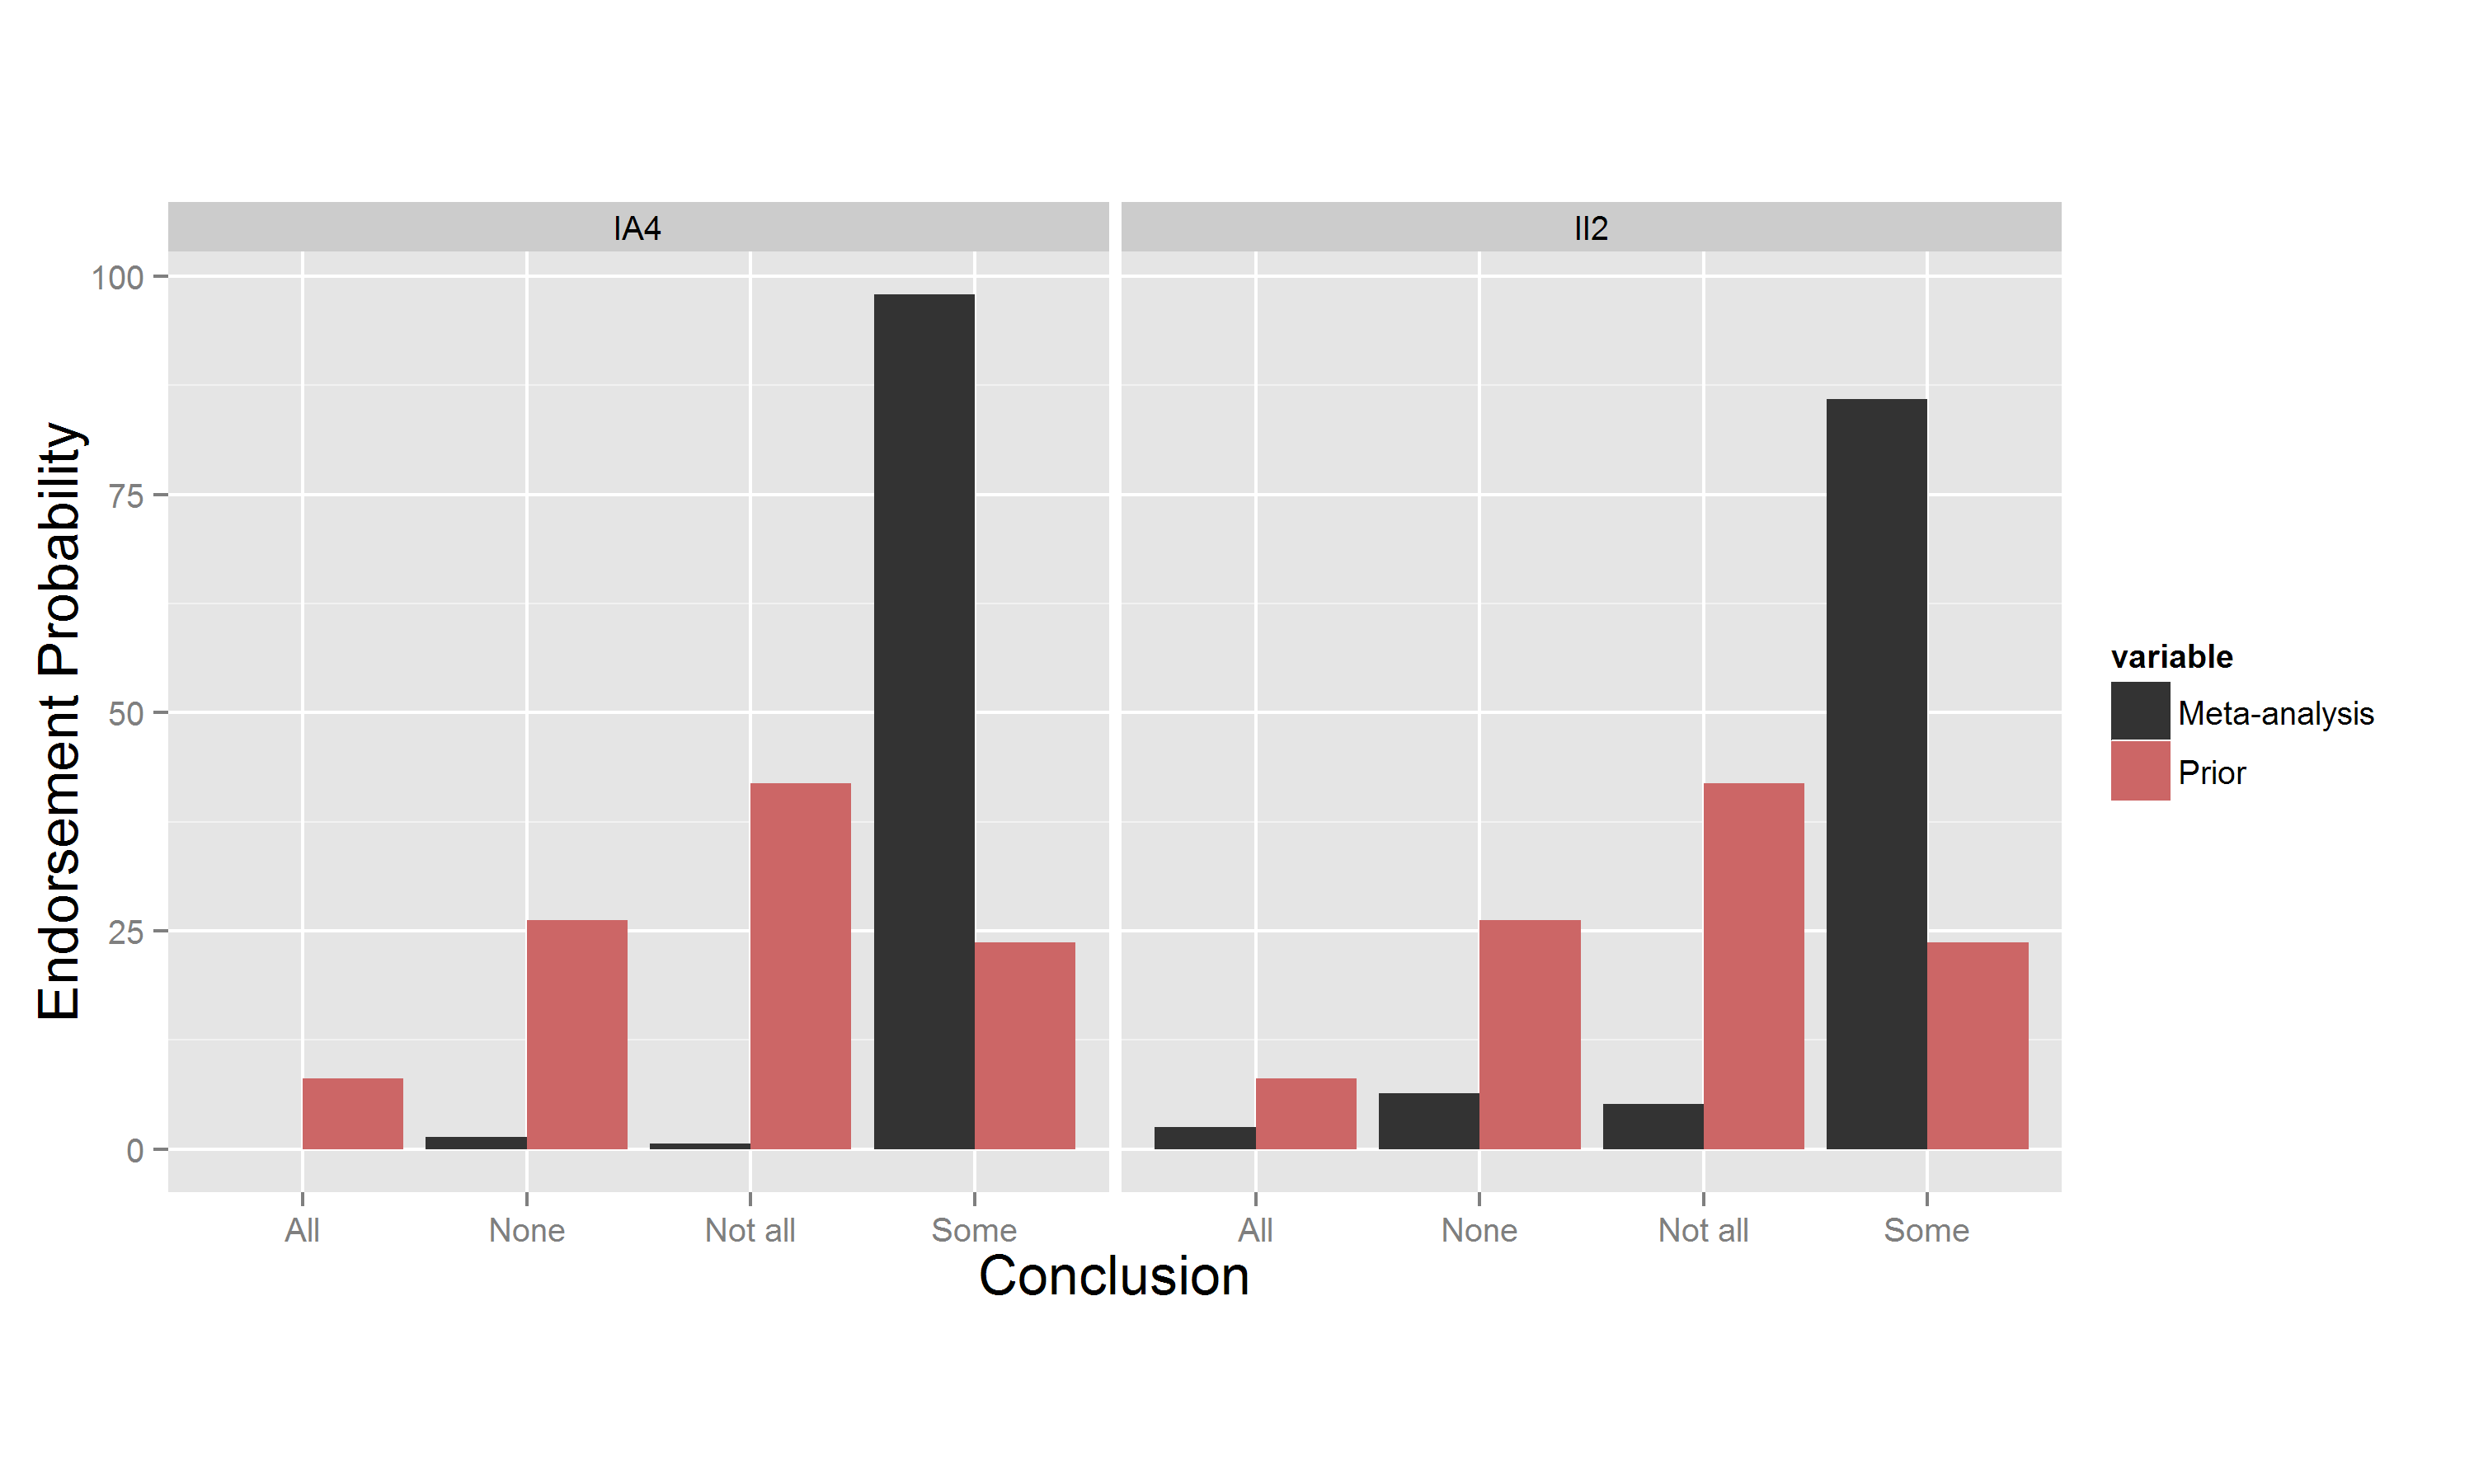
\includegraphics[width = {0.66\columnwidth}]{multibar_alpha1_prior}
%	\label{fig:subfigure1}}
%%\caption{Single-model, valid}}
%%\hfill
%\subfigure[conditional semantics]{ %}
%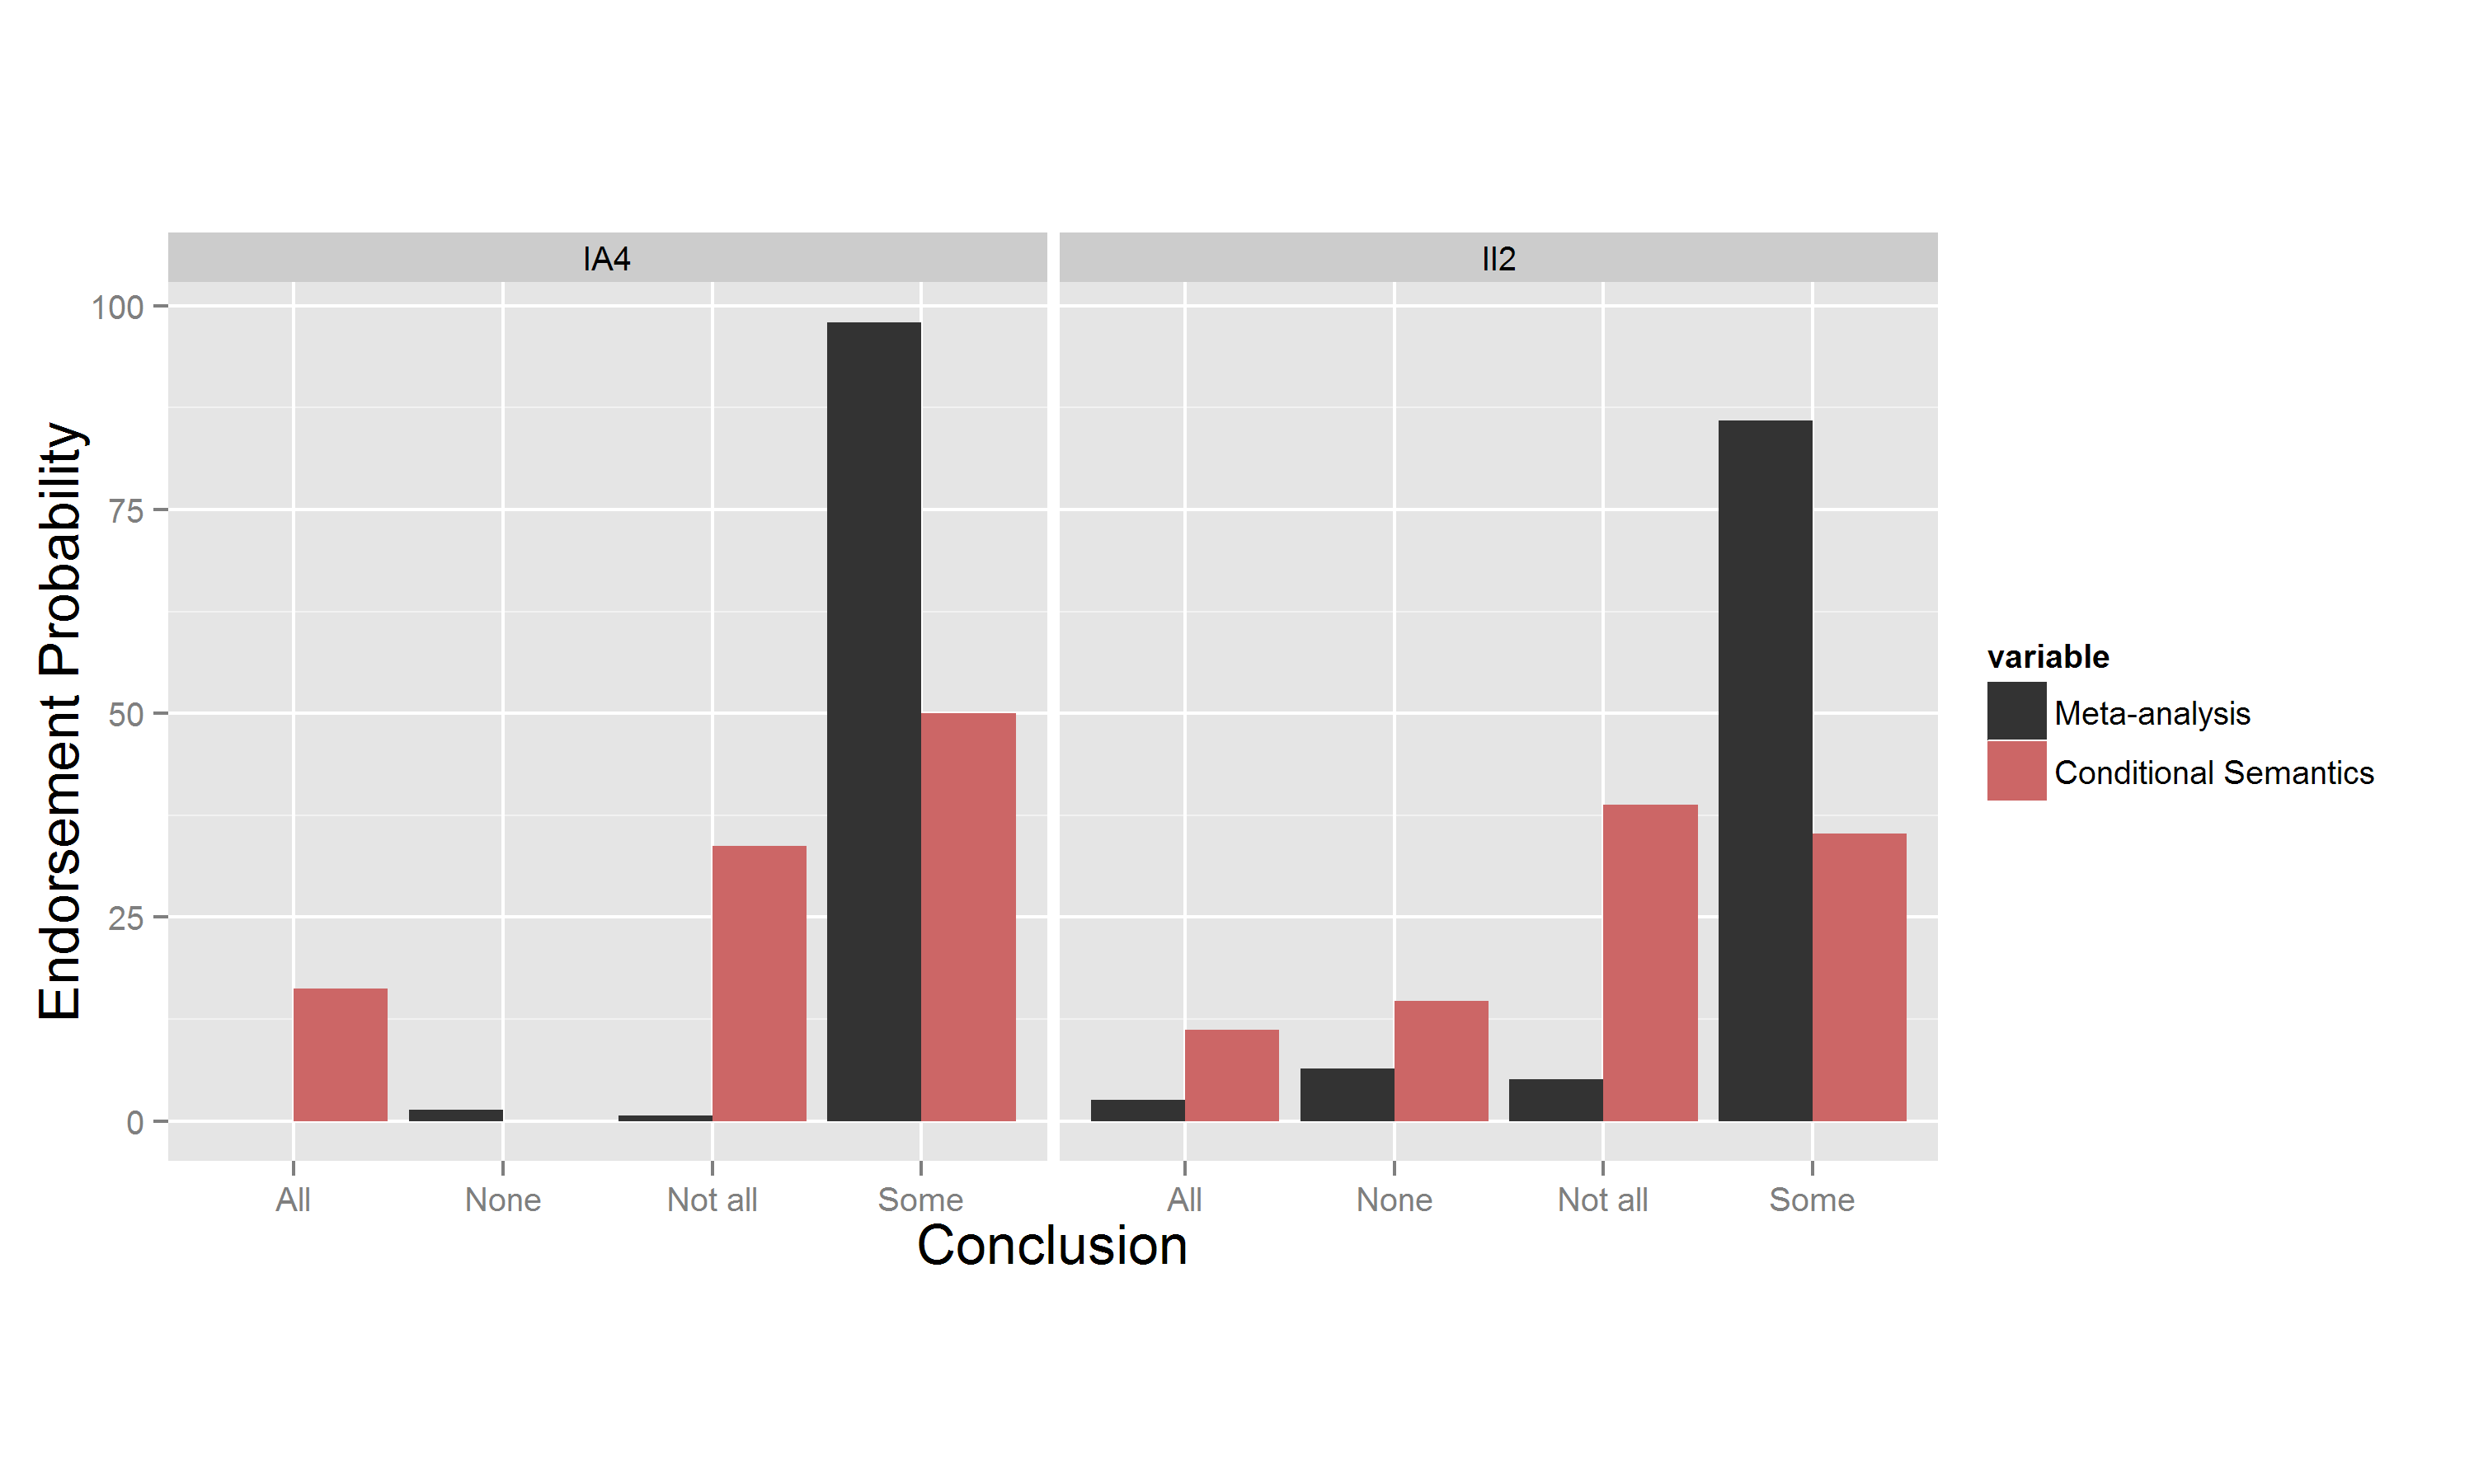
\includegraphics[width = {0.66\columnwidth}]{multibar_alpha1_lit}
%%\label{fig:subfigure3}
%\caption{Multiple-model, valid}
%}
%%\hfill
%\subfigure[conditional pragmatics]{
%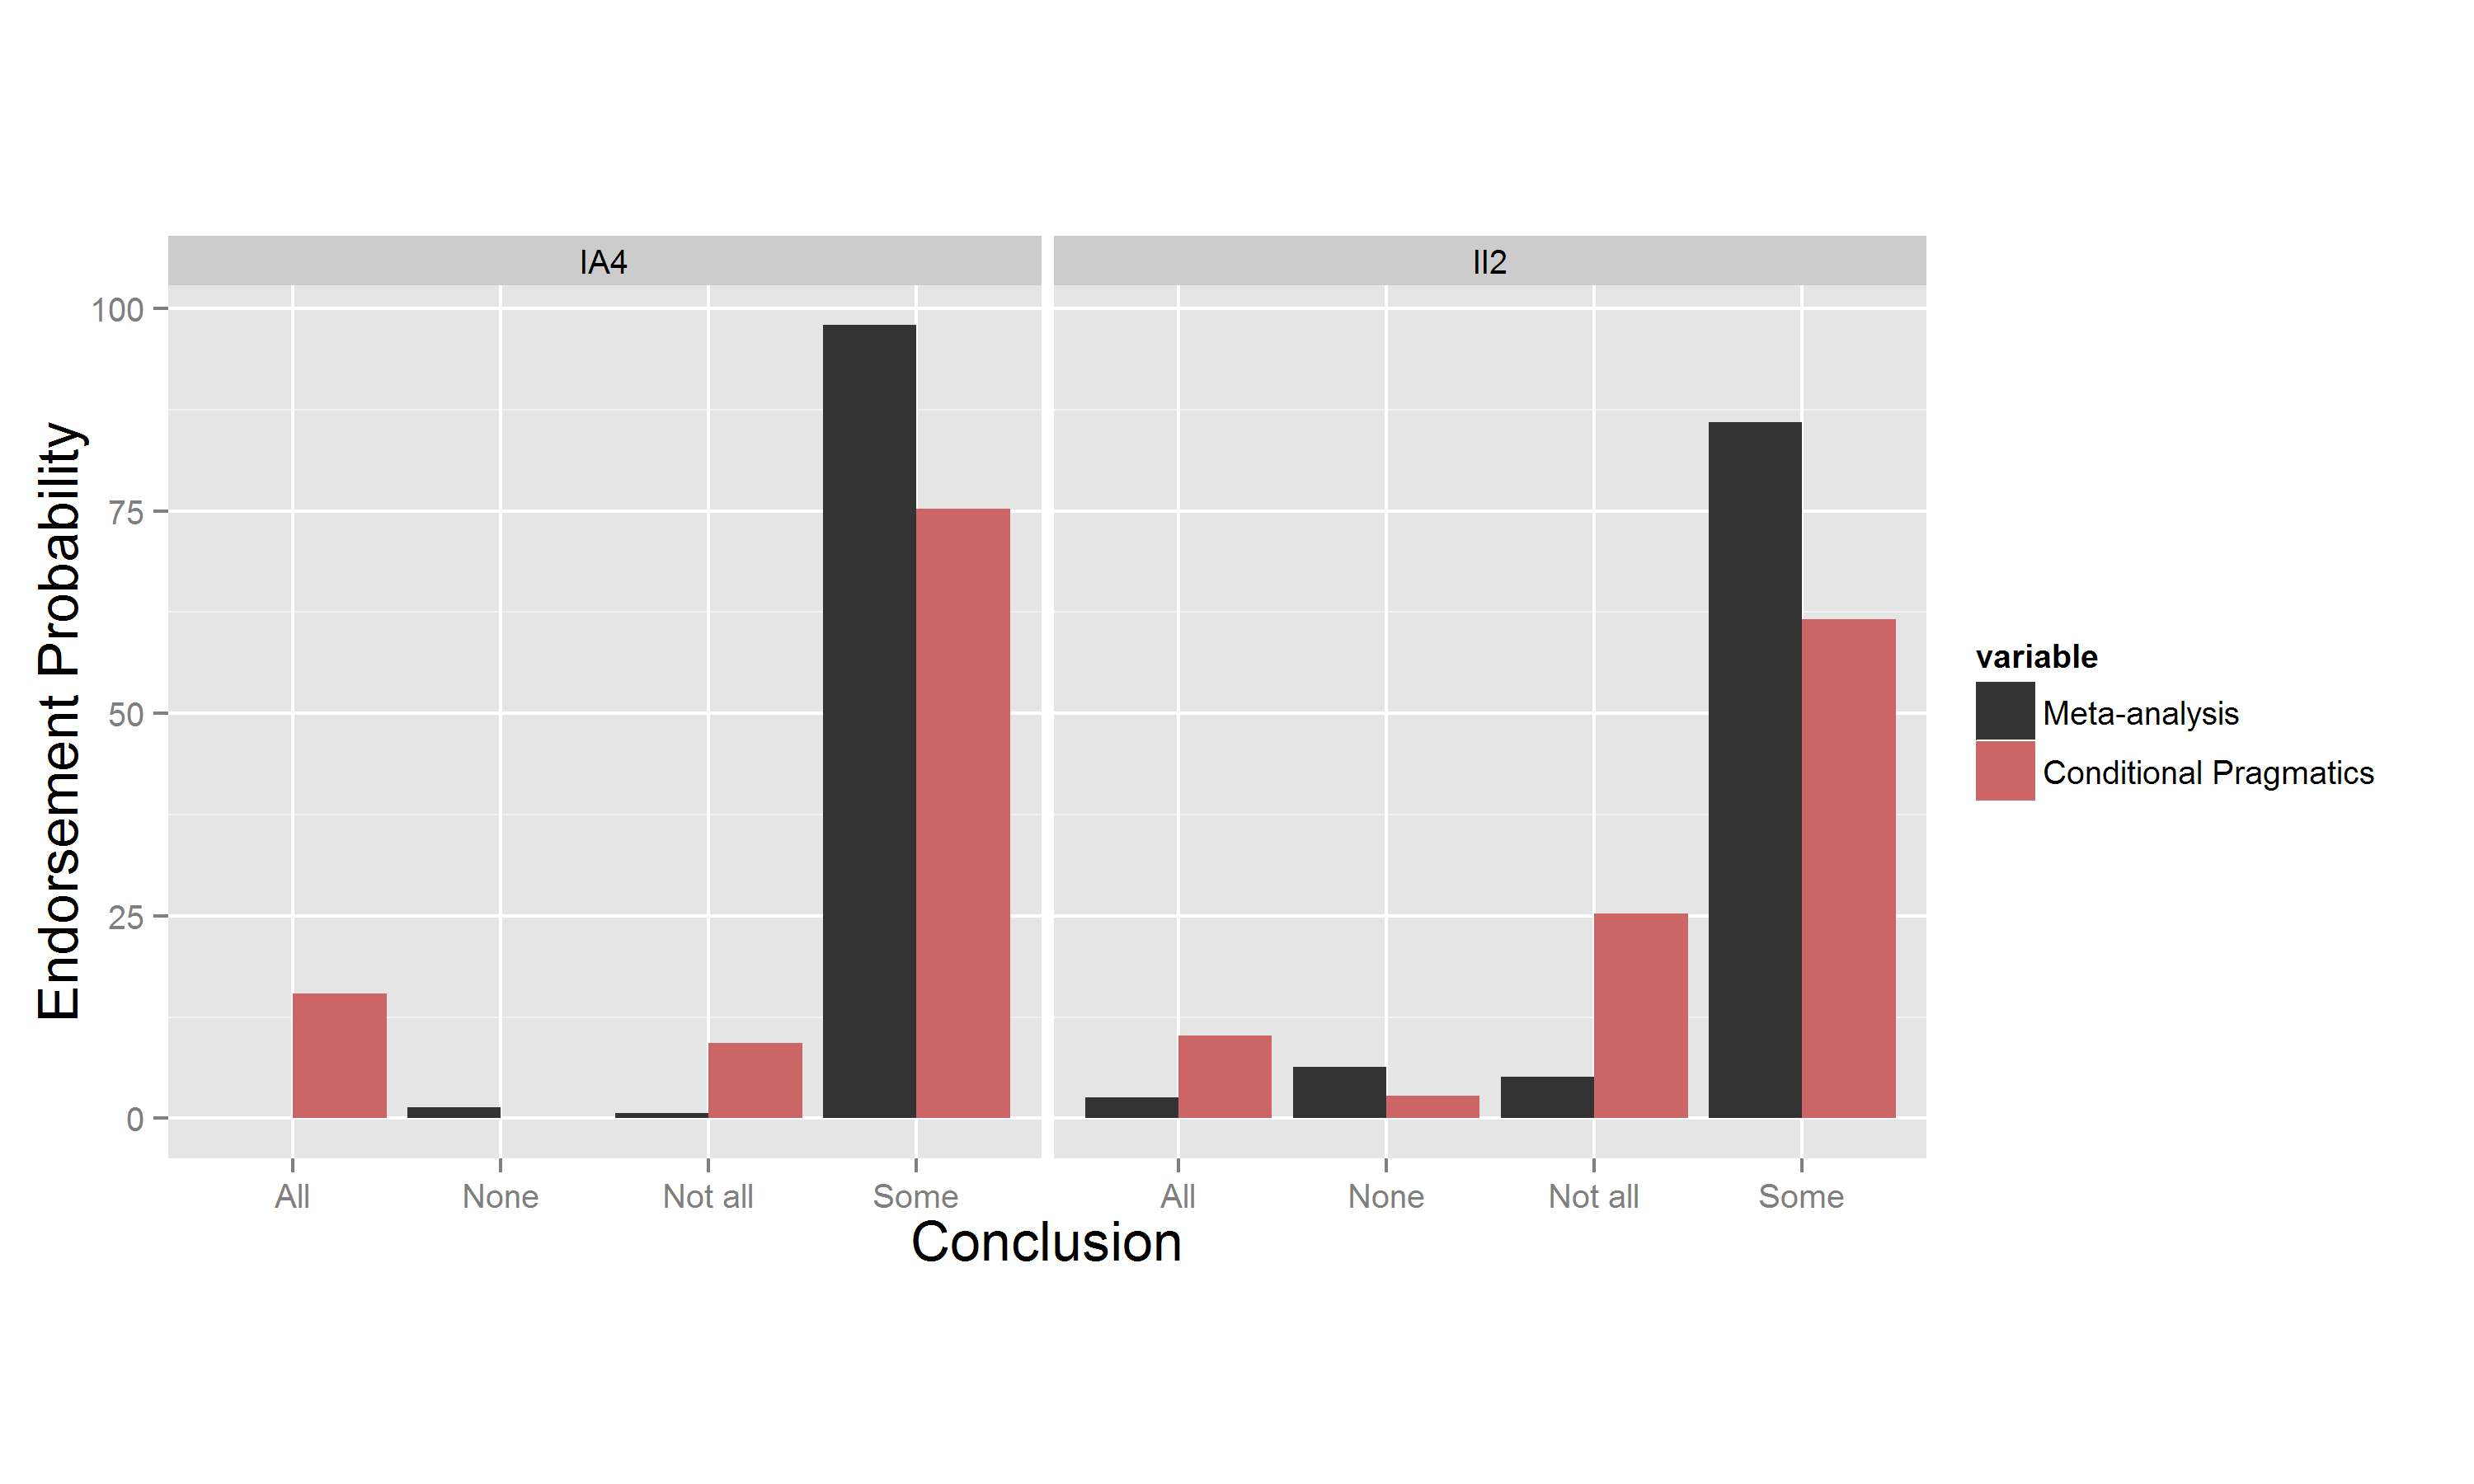
\includegraphics[width = {0.66\columnwidth}]{multibar_alpha1_prag}
%%\label{fig:subfigure5}
%\caption{invalid}
%%}
%%\quad
%%
%%\subfigure[one model, valid]{ %
%%\includegraphics[width = {0.66\columnwidth}]{IA4_boxplot_text}
%%%\label{fig:subfigure2}}
%%\hfill
%%\subfigure[multiple models, valid]{
%%\includegraphics[width = {0.66\columnwidth}]{EI3_boxplot_text}
%%%\label{fig:subfigure4}}
%%\caption{Multiple-model, valid}
%%\hfill
%%\subfigure[invalid]{
%%\includegraphics[width = {0.66\columnwidth}]{AA2_boxplot_text}
%%%\label{fig:subfigure6}}
%%\caption{invalid}
%%
%%\caption{Participants' endorsements in six syllogisms}
%%\label{fig:fig1}


%
%
%Mental Models Theory explains difficulty in syllogisms by demonstrating that multiple, distinct situations can be consistent with a pair of premises, giving rise to different possible conclusions. Valid syllogistic conclusions arise in every possible model. (This is the same notion of Pr(conclusion | premises) = 1). 
%
%This is always the case the logically invalid syllogisms (see discussion below), and is sometimes the case with logically valid syllogisms.

%\subsubsection{Logical invalidity}
%For syllogisms that have no valid conclusion, the probabilistic reasoner computes the probability of the conclusion conditioned on the premises being true by sampling. For all invalid syllogisms, this yield a gradeds response across the different possible conclusion types. 
%
%
%\subsubsection{Logical validity}
%A conclusion is logically valid if and if only it is true in all possible situations. Recall that possible situations are restricted to those that are consistent with the premises. The universal quantifiers (all, none) entail their particular counterparts (some, not-all), respectively. This was noticed by Aristotle and commonly visualized in the \emph{Square of Opposition}. For our probabilistic reasoner, confidence for {\emph all} and {\emph some} (to take the affirmative case) will be both maximal. {\emph All} is always true and {\emph some} is true whenever {\emph all} is true.


%We tested a number of rarity factors and found that p=0.25 provided the best fit. This is also consistent with the Probability Heuristic's rarity assumption. 


%\red{math here?}

%For reasoning over syllogisms, the prior distribution is conditioned on the truth of the premise sentences. This is the distribution over sentences conditioned on the fact that the premises are true. In this way, we evaluate the $\Pr$(conclusion $\arrowvert$ premises). This is essentially a metric of the plausibility of the argument. In this formulation, $\Pr$(conclusion $\arrowvert$ premises) = 1 if and only if the syllogism is logically valid.

%
%To set this parameter, we follow Johnson-Laird's principle of parsimony, which states that situations are constructed to ``maximize the number of properties of each individual to try to keep the number of \emph{distinct sorts} of individuals to a minimum".
%
%, from which we accept only those consistent with the premises \footnote{We follow J-L's lead by imposing the additionasl constraint that the syllogistic terms refer to non-empty classes in the world. This is the existential presupposition.}.
%
%The basic model has two parameters, which both contribute to the concept of Expected Value: situation size and property rarity. We tested a number of situation sizes and found 6 to be the best. This is consistent with Johnson-Laird's principle of parsimony which states that models are constructed to ``maximize the number of properties of each individual to try to keep the number of \emph{distinct sorts} of individuals to a minimum". 
%
%The number of distinct sorts of individuals is highest for logically invalid syllogisms precisely because the problems are not fully constrained. In Johnson-Laird's examples of these types of models, the number of individuals is always 6. 
%
%Rarity refers to the probability that a particular object in a world has a property (or belongs to class). A principle of rarity is often assumed in line with the intuition that properties are relative rare \footnote{This article is an article and it's about reasoning, but it's not a cat, and it's not a car, nor an elephant nor the color red. In fact, there's a very large number of things which this article is not.}, and we assume a principle of rarity here. We tested a number of rarity factors and found that p=0.25 provided the best fit. This is also consistent with Chater \& Oaksford's rarity assumption. 

%\subsection{Model predictions}

\

\bibliographystyle{apacite}

\setlength{\bibleftmargin}{.125in}`
\setlength{\bibindent}{-\bibleftmargin}

\bibliography{mhtbib}


\end{document}



TODO after cogsci:
-implement phm (and mm?) for comparison.
-understand alpha param and pragmatic production recursion depth.
-understand the origin of symmetry breaking in 'prior' (i.e. funny prior which should be pragmatic).
-understand why pragmatic comprehender model doesn't work.
-analyze errors better.
-do experiments to get estimate of priors.
